%; whizzy paragraph -pdf xpdf -latex ./whizzypdfptex.sh
%; whizzy-paragraph "^\\\\begin{frame}\\|\\\\emtext"
% latex beamer presentation.
% platex, latex-beamer でコンパイルすることを想定。 

%     Tokyo Debian Meeting resources
%     Copyright (C) 2012 Junichi Uekawa

%     This program is free software; you can redistribute it and/or modify
%     it under the terms of the GNU General Public License as published by
%     the Free Software Foundation; either version 2 of the License, or
%     (at your option) any later version.

%     This program is distributed in the hope that it will be useful,
%     but WITHOUT ANY WARRANTY; without even the implied warreanty of
%     MERCHANTABILITY or FITNESS FOR A PARTICULAR PURPOSE.  See the
%     GNU General Public License for more details.

%     You should have received a copy of the GNU General Public License
%     along with this program; if not, write to the Free Software
%     Foundation, Inc., 51 Franklin St, Fifth Floor, Boston, MA  02110-1301 USA

\documentclass[cjk,dvipdfmx,12pt]{beamer}
\usetheme{Tokyo}
\usepackage{monthlypresentation}

%  preview (shell-command (concat "evince " (replace-regexp-in-string "tex$" "pdf"(buffer-file-name)) "&")) 
%  presentation (shell-command (concat "xpdf -fullscreen " (replace-regexp-in-string "tex$" "pdf"(buffer-file-name)) "&"))
%  presentation (shell-command (concat "evince " (replace-regexp-in-string "tex$" "pdf"(buffer-file-name)) "&"))

%http://www.naney.org/diki/dk/hyperref.html
%日本語EUC系環境の時
\AtBeginDvi{\special{pdf:tounicode EUC-UCS2}}
%シフトJIS系環境の時
%\AtBeginDvi{\special{pdf:tounicode 90ms-RKSJ-UCS2}}

\newenvironment{commandlinesmall}%
{\VerbatimEnvironment
  \begin{Sbox}\begin{minipage}{1.0\hsize}\begin{fontsize}{8}{8} \begin{BVerbatim}}%
{\end{BVerbatim}\end{fontsize}\end{minipage}\end{Sbox}
  \setlength{\fboxsep}{8pt}
% start on a new paragraph

\vspace{6pt}% skip before
\fcolorbox{dancerdarkblue}{dancerlightblue}{\TheSbox}

\vspace{6pt}% skip after
}
%end of commandlinesmall

\title{東京エリアDebian勉強会\\Debianパッケージング道場}
\subtitle{第130回 2015年9月度}
\author{岩松 信洋}
\date{2015年9月12日}
\logo{
\includegraphics[width=8cm]{image200607/openlogo-light.eps}}

\begin{document}

\begin{frame}
\titlepage{}
\end{frame}

\begin{frame}{設営準備にご協力ください。}
会場設営よろしくおねがいします。
\end{frame}

\begin{frame}{Agenda}
\begin{itemize}
   \item 最近あったDebian関連のイベント報告
	 \begin{itemize}
	 \item 第129回 東京エリアDebian勉強会
	 \item OSC 2015 Niigata
	 \end{itemize}
   \item パッケージングチュートリアルを使った解説
   \item パッケージング道場
   \item 今後のイベント
   \item 今日の宴会場所
  \end{itemize}
\end{frame}

\section{イベント報告}
\emtext{イベント報告}

\begin{frame}{第129回東京エリアDebian勉強会}

\begin{itemize}
\item 場所はスクウェア・エニックスさんのセミナルームをお借りしての開催でした。
\item セミナは野島さんによる「APT1.1 超☆牛さんパワー炸裂!」と題した APT 1.1 の解説でした。
\item 残りの時間でhack timeを行い、成果発表をしました。
\end{itemize} 
\end{frame}

\begin{frame}{OSC 2015 Niigata}

\begin{itemize}
\item 9/8 に 新潟でOSCが開催され、野島さんと吉田さんがさんかされました。\url{/http://www.ospn.jp/osc2015-niigata/}
\item セミナと展示を行い、セミナーは野島さんによる「Debian update」と題した Debian 8.0 の紹介が行われました。
\end{itemize} 

\end{frame}

\section{Debian パッケージング道場}
\emtext{Debian パッケージング道場}

\begin{frame}{本日の流れ}

\begin{itemize}
 \item 午前の部
  \begin{itemize}
   \item パッケージングチュートリアルを使った Debian パッケージの解説
   \item git buildpackage の使い方を解説
  \end{itemize}
 \item お昼ごはん
 \item 午後の部 (13:00 -)
  \begin{itemize}
   \item パッケージ作業
   \item 成果報告
  \end{itemize}
\end{itemize}

\end{frame}

\emtext{パッケージングチュートリアル}
\emtext{git buildpackage}

\begin{frame}

Debian パッケージングチュートリアルであまり解説されていない gbp (git
buildpackage) の基本的な使い方について説明する。

\end{frame}

\begin{frame}{VCS で管理しない場合}

\begin{center}
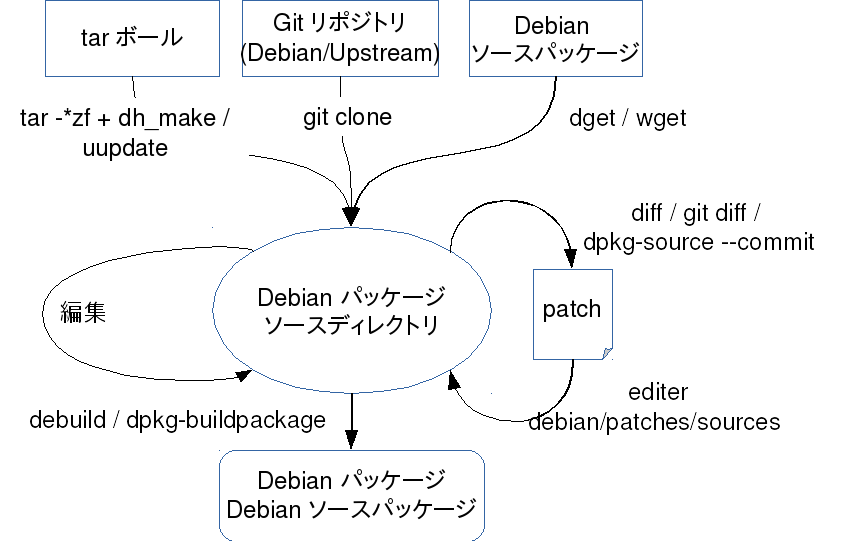
\includegraphics[width=0.8\hsize]{image201509/gbp-images0.png}
\end{center}

\end{frame}

\begin{frame}{VCS で管理する場合}
\begin{center}
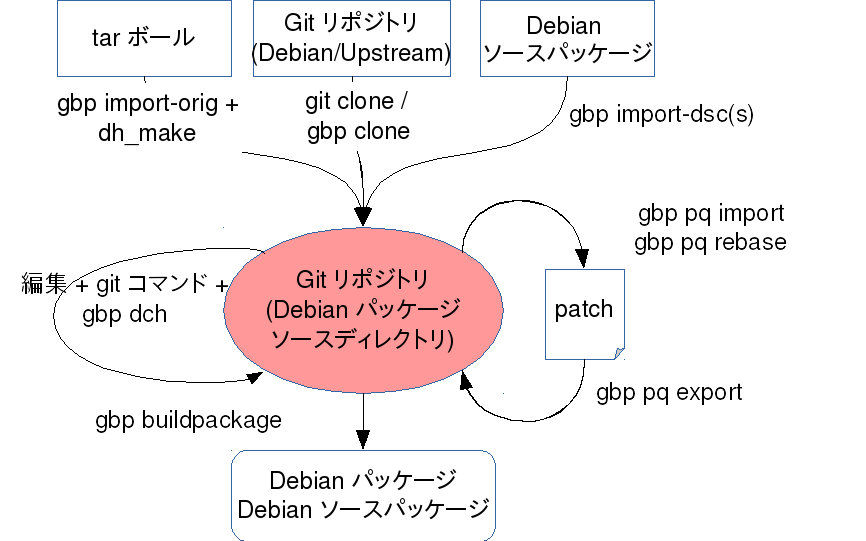
\includegraphics[width=0.8\hsize]{image201509/gbp-images1.png}
\end{center}
\end{frame}

\begin{frame}[containsverbatim]{Upstream から tar ボールがリリースされている場合}

Upstream からtarボールがリリースされている場合、
tar ボールをGitリポジトリにコミットした後、パッケージ化を行う。

\end{frame}

\begin{frame}[containsverbatim]
\begin{itemize}
\item tar ボールをダウンロードする

\begin{commandline}
$ wget package-name-0.0.1.tar.gz
\end{commandline}

\item Gitリポジトリを作成する

\begin{commandline}
$ git init package-name
$ cd package-name
\end{commandline}

必要であれば git config で Git の設定を変更する。
\end{itemize}
\end{frame}

\begin{frame}[containsverbatim]
\begin{itemize}
\item tar ボールを指定して、ソースコードを Git にコミットする

\begin{commandline}
$ gbp import-orig --pristine-tar \
	../package-name-0.0.1.tar.gz
$ git tag 
$ upstream/0.0.1
$ git branch
* master
  upstream
\end{commandline}
\end{itemize}
\end{frame}

\begin{frame}[containsverbatim]
\begin{itemize}
\item Upstreamのコードをは upstream ブランチで管理され、同時にタグが設
定される。
\item pristine-tar オプションはオリジナルのtarボールの差分を保存するための仕組みを有効
にする。Upstreamのコードは upstream ブランチで管理され、Debian パッケージを
作成するときに、そこから orig.tar.gz ファイルを作成する。この時に作成されるファイル
が同じものにならない場合がある。Debian では
取り込んだ tat.gz ファイルのハッシュ値とDebian ソースパッケージとしてアップロードされる
tar.gz ファイルが同じである必要があるため、本オプションを用いて orig.tar.gzとの差分を
バイナリパッチとして保存し、orig.tar.gzを構築する度に再適用することで、ハッシュ値
が同じorig.tar.gzを再構築できるようにしている。
\end{itemize}
\end{frame}

\begin{frame}[containsverbatim]
\begin{itemize}
\item dh\_make で debian ディレクトリの雛形を作成する 

\begin{commandline}
$ dh_make -p package-name_0.0.1
\end{commandline}

\item debian ディレクトリ内をいろいろ変更する

\begin{commandline}
$ いろいろ修正
$ git add debian
$ git commit
\end{commandline}
\end{itemize}
\end{frame}

\begin{frame}[containsverbatim]
\begin{itemize}
\item パッケージ化作業ができたら パッケージを構築する

\begin{commandline}
$ gbp buildpackage --git-pristine-tar
\end{commandline}

\item piuparts などでインストール、アンインストールのテスト

\item 最後にクリーンな環境でビルドテスト

\begin{commandline}
$ git-pbuilder
or
$ gbp buildpackage --git-pbuiler --git-pristine-tar
\end{commandline}
\end{itemize}
\end{frame}

\begin{frame}[containsverbatim]
\begin{itemize}
\item タグを設定して リモートリポジトリにプッシュする

\begin{commandline}
$ gbp buildpackage --git-tag-only
$ git push
\end{commandline}

\end{itemize}
\end{frame}

\begin{frame}{upstream に更新があった場合}

\end{frame}

\begin{frame}[containsverbatim]
\begin{itemize}
\item upstream のtar ボールを取得する

\begin{commandline}
$ wget package-name-0.0.2.tar.gz
\end{commandline}

\item tar ボールを指定してリポジトリにソースコードをコミットする

\begin{commandline}
$ gbp import-orig --pristine-tar \
		../package-name-0.0.2.tar.gz
\end{commandline}

\texttt{--uscan} オプションでダウンロード $\rightarrow$ コミットが一度にできる。
また、ソースコードは自動的にマージされます。マージしたくない場合は
\texttt{--no-merge} を指定して実行する。
\end{itemize}
\end{frame}

\begin{frame}[containsverbatim]
\begin{itemize}
\item debian/changelog を修正

\begin{commandline}
$ dch -i
or
$ gbp dch 
\end{commandline}

\item パッケージをビルド

\begin{commandline}
$ gbp buildpackage --git-pristine-tar \
		--git-pristine-tar-commit
\end{commandline}

\end{itemize}

\end{frame}

% -------------------------------------------------

\begin{frame}[containsverbatim]{Upstream が Git で管理されている場合}

\begin{itemize}
\item  Upstream では tar ボールでリリースされず、Gitのタグのみでリリースされる場合
もある。
\item Github で開発されているプロジェクトが良い例。
\item このような場合は リポジトリをクローンした後、Debian独自のブランチルールを用いて
ソースパッケージの管理を行う。
\end{itemize}

\end{frame}

\begin{frame}[containsverbatim]
\begin{itemize}

\item リポジトリをクローンし、作成されたディレクトリに移動する

\begin{commandline}
$ git clone git://example.org/git/package-name.git
$ cd package-name
\end{commandline}
\end{itemize}
\end{frame}

\begin{frame}[containsverbatim]
\begin{itemize}
\item ベースにしたいバージョンのコードをチェックアウトする

\begin{commandline}
$ git reset --hard 0.0.1
\end{commandline}
\end{itemize}
\end{frame}

\begin{frame}[containsverbatim]
\begin{itemize}
\item タグを設定する

\begin{commandline}
$ git tag upstream/0.0.1
\end{commandline}

upstream ネームスペースは gbp デフォルト参照先。Upstreamのタグを使いたい場合
や独自のネームスペースを使いたい場合は gbp の upstream-tag が利用できます。

\begin{commandline}
[git-buildpackage]
upstream-tag = v%(version)s
\end{commandline}
\end{itemize}
\end{frame}

\begin{frame}[containsverbatim]
\begin{itemize}
\item dh\_make で debian ディレクトリの雛形を作成する

\begin{commandline}
$ dh_make -p package-name_0.0.1
\end{commandline}
\end{itemize}
\end{frame}

\begin{frame}[containsverbatim]
\begin{itemize}
\item debian ディレクトリ内をいろいろ変更する

\begin{commandline}
$ いろいろ修正
$ git add debian
$ git commit
\end{commandline}
\end{itemize}
\end{frame}

\begin{frame}[containsverbatim]
\begin{itemize}
\item パッケージ化作業ができたら パッケージを構築する

\begin{commandline}
$ gbp buildpackage --git-pristine-tar \
		--git-pristine-tar-commit
\end{commandline}

tar ボールを使う場合と異なるのは\texttt{--git-pristine-tar-commit} オプション
を指定すること。このオプションを指定することによってタグから orig.tar.gz を生成
する。
\end{itemize}
\end{frame}

\begin{frame}[containsverbatim]
\begin{itemize}
\item piuparts などでインストール、アンインストールのテスト

\item 最後にクリーンな環境でビルドテスト

\begin{commandline}
$ git-pbuilder
or
$ gbp buildpackage --git-pbuilder
\end{commandline}
\end{itemize}
\end{frame}

\begin{frame}[containsverbatim]
\begin{itemize}
\item タグを設定して リモートリポジトリにプッシュする

\begin{commandline}
$ gbp buildpackage --git-tag-only
$ git push
\end{commandline}

\end{itemize}
\end{frame}

\begin{frame}{upstream に更新があった場合}

\end{frame}

\begin{frame}[containsverbatim]
\begin{itemize}
\item upstream のリポジトリ情報を取得する

\begin{commandline}
$ git remote update
\end{commandline}
\end{itemize}
\end{frame}

\begin{frame}[containsverbatim]
\begin{itemize}
\item 変更をマージ

\begin{commandline}
$ git tag upstream/0.0.2 0.0.2
$ git merge upstream/0.0.2
\end{commandline}
\end{itemize}
\end{frame}

\begin{frame}[containsverbatim]
\begin{itemize}
\item debian/changelog を修正

\begin{commandline}
$ dch -i
or
$ gbp dch
\end{commandline}
\end{itemize}
\end{frame}

\begin{frame}[containsverbatim]
\begin{itemize}
\item パッケージをビルド

\begin{commandline}
$ gbp buildpackage --git-pristine-tar\
		--git-pristine-tar-commit
\end{commandline}

\end{itemize}
\end{frame}

\begin{frame}{アップストリームのソースコード変更}

\begin{enumerate}
\item gbp pq import
\item Upstream ソースコードの修正
\item git commit
\item gbp pq export
\item git commit
\end{enumerate}

\end{frame}

\begin{frame}

\begin{center}
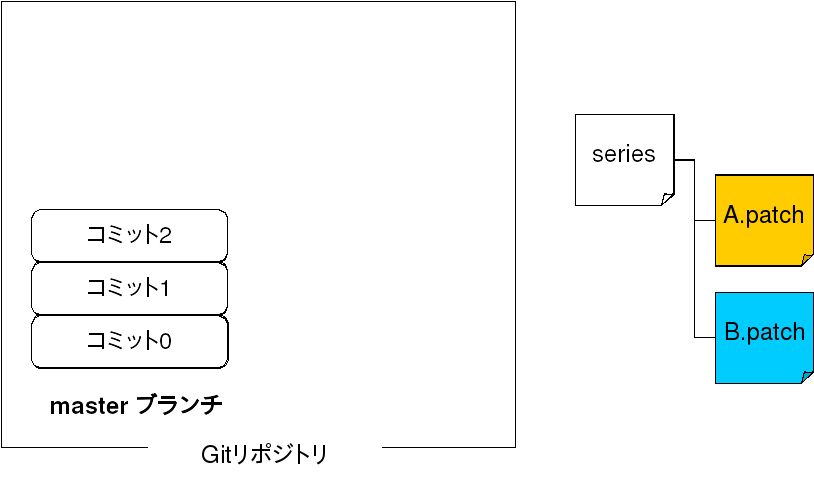
\includegraphics[width=0.8\hsize]{image201509/gbp-pq0.png}
\end{center}

\end{frame}

\begin{frame}{gbp pq import}

  \begin{enumerate}
   \item HEAD をpatch-queue/master ブランチとしてチェックアウト
   \item debian/patches/series にあるパッチをコミット
  \end{enumerate}

\begin{center}
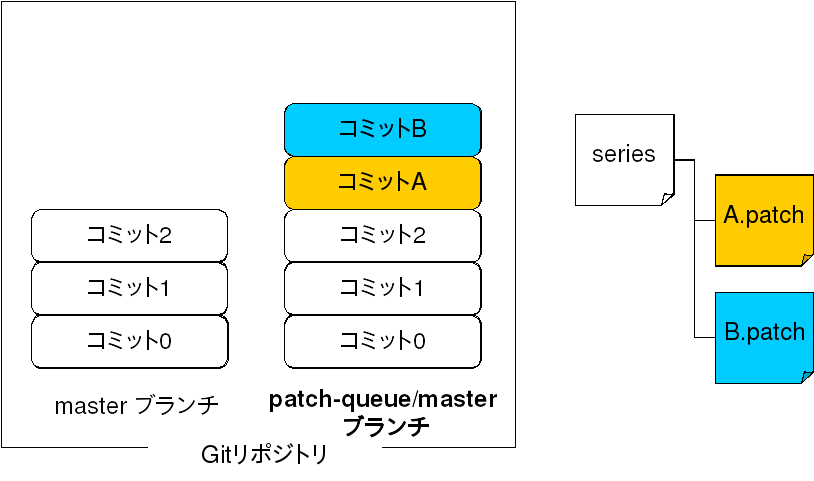
\includegraphics[width=0.8\hsize]{image201509/gbp-pq1.png}
\end{center}

\end{frame}

\begin{frame}{修正 \& git commit}

  \begin{enumerate}
   \item Upstream ソースコードの修正
   \item git commit
  \end{enumerate}

\begin{center}
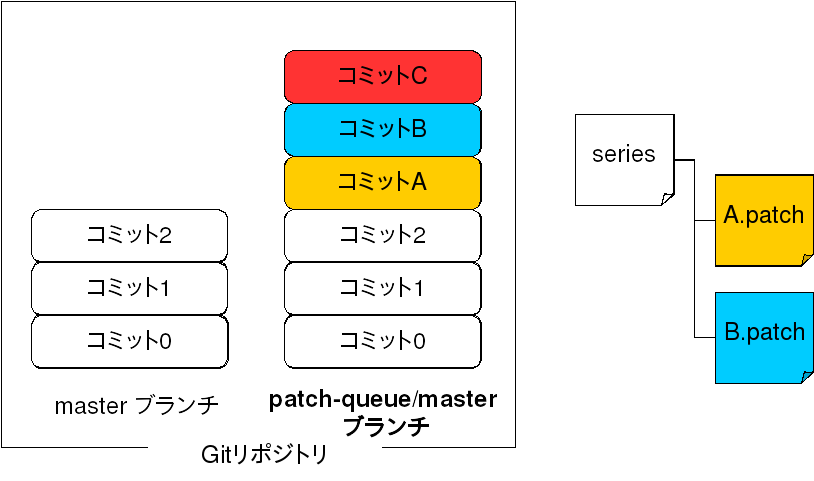
\includegraphics[width=0.8\hsize]{image201509/gbp-pq2.png}
\end{center}

\end{frame}

\begin{frame}{gbp pq export}
  \begin{enumerate}
   \item patch-queue/master と master ブランチの差分をパッチとして debian/patches に出力
   \item debian/patches/series を更新
   \item master ブランチをチェックアウト
  \end{enumerate}

\begin{center}
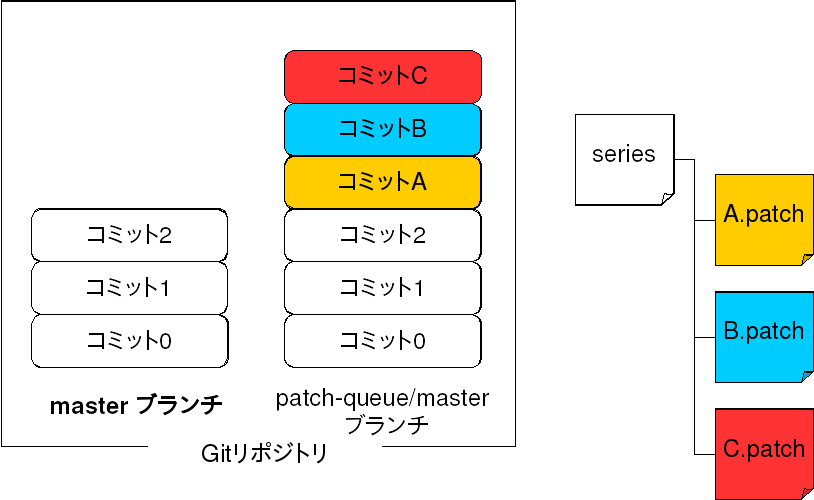
\includegraphics[width=0.8\hsize]{image201509/gbp-pq3.png}
\end{center}
  
  
\end{frame}

\begin{frame}{git commit}
  \begin{enumerate}
   \item パッチ更新をリポジトリにコミット
  \end{enumerate}

\begin{center}
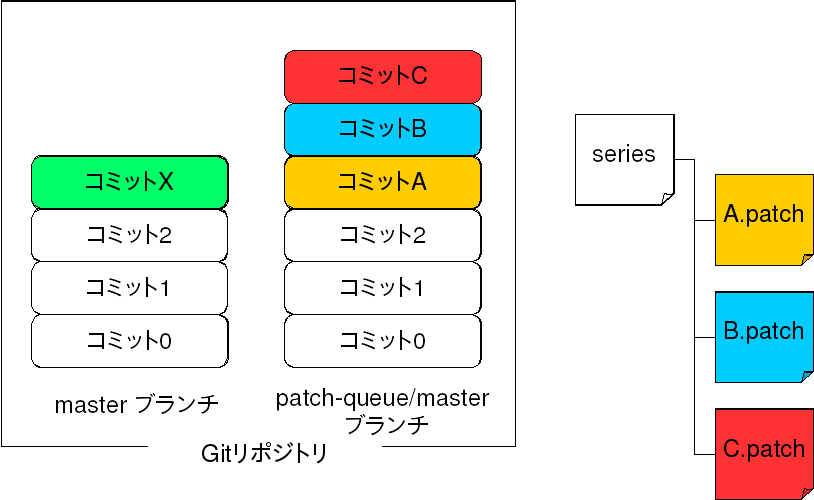
\includegraphics[width=0.8\hsize]{image201509/gbp-pq4.png}
\end{center}
\end{frame}

\begin{frame}{まとめ}

\begin{itemize}
\item gbp (git buildpackage)はデファクトスタンダート
\item gbp import-* でリポジトリ取り込み
  
  \texttt{--pristine-tar} を忘れずに
\item gbp dch で debian/changelog を更新
\item gbp buildpackage でパッケージビルド
\item gbp pq でパッチ操作
\end{itemize}


\end{frame}

\emtext{パッケージ作業}
\emtext{成果報告}

\section{今後のイベント}
\emtext{今後のイベント}
\begin{frame}{今後のイベント}
\begin{itemize}
 \item 関西エリアDebian勉強会
 \item 10/24(土)、10/25(日) OSC 2015 Tokyo Fallでセミナ&ブース\\
\url{http://www.ospn.jp/osc2015-fall/}
\end{itemize}
\end{frame}

\section{今日の宴会場所}
\emtext{今日の宴会場所}
\begin{frame}{今日の宴会場所}
未定
\end{frame}

\end{document}

;;; Local Variables: ***
;;; outline-regexp: "\\([ 	]*\\\\\\(documentstyle\\|documentclass\\|emtext\\|section\\|begin{frame}\\)\\*?[ 	]*[[{]\\|[]+\\)" ***
;;; End: ***
